\documentclass[conference]{IEEEtran}
\IEEEoverridecommandlockouts
\usepackage{cite}
\usepackage{amsmath,amssymb,amsfonts}
\usepackage{graphicx}
\usepackage{textcomp}
\usepackage{xcolor}
\usepackage{array}
\usepackage{booktabs}
\usepackage[hidelinks]{hyperref}
\newcolumntype{L}[1]{>{\raggedright\arraybackslash}p{#1}}
\graphicspath{{figures/}}
\hyphenation{Py-thon data-set Play-wright}
% Latin Modern for monospaced and sans text: the local TeX install has Times but not Courier or Helvetica.
% On Overleaf or a full TeX Live these two lines can be removed to get IEEEtran's default Courier.
\renewcommand{\ttdefault}{lmtt}
\renewcommand{\sfdefault}{lmss}

% Four authors in a two-by-two grid (IEEEtran conference mode).
\makeatletter
\newcommand{\linebreakand}{%
  \end{@IEEEauthorhalign}
  \hfill\mbox{}\par
  \mbox{}\hfill\begin{@IEEEauthorhalign}
}
\makeatother

\begin{document}

\title{Smart Telecom Revenue \& Churn Command Center: A Dual-Engine Operations Research Optimization Suite}

\author{
\IEEEauthorblockN{Deep Amit Lodaya}
\IEEEauthorblockA{CB.AI.U4AID23004\\
\textit{Amrita School of Artificial Intelligence}\\
\textit{Amrita Vishwa Vidyapeetham}\\
Coimbatore, Tamil Nadu, India\\
cb.ai.u4aid23004@cb.students.amrita.edu}
\and
\IEEEauthorblockN{Harigovind Krishnan}
\IEEEauthorblockA{CB.AI.U4AID23010\\
\textit{Amrita School of Artificial Intelligence}\\
\textit{Amrita Vishwa Vidyapeetham}\\
Coimbatore, Tamil Nadu, India\\
cb.ai.u4aid23010@cb.students.amrita.edu}
\linebreakand
\IEEEauthorblockN{Vimal P Menon}
\IEEEauthorblockA{CB.AI.U4AID23050\\
\textit{Amrita School of Artificial Intelligence}\\
\textit{Amrita Vishwa Vidyapeetham}\\
Coimbatore, Tamil Nadu, India\\
cb.ai.u4aid23050@cb.students.amrita.edu}
\and
\IEEEauthorblockN{Dasigi Prasanna Jagannath}
\IEEEauthorblockA{CB.AI.U4AID23065\\
\textit{Amrita School of Artificial Intelligence}\\
\textit{Amrita Vishwa Vidyapeetham}\\
Coimbatore, Tamil Nadu, India\\
cb.ai.u4aid23065@cb.students.amrita.edu}
}

\maketitle

\begin{abstract}
Telecom operators usually set prices and fund retention campaigns as separate decisions, yet both act on the same quantity: how long a customer stays. This paper presents the Smart Telecom Revenue \& Churn Command Center, a web application that treats the two decisions as linked optimization problems on the IBM Telco customer churn dataset of 7,043 subscribers. A least-squares fit recovers a ten-service price list from unitemized bills ($R^2 = 0.9988$), and a piecewise-exponential Poisson model turns the churn label into a monthly hazard for every customer. Engine~1, a nonlinear program solved by sequential quadratic programming, reprices the ten services under price bounds, a $\pm 15\%$ bill-shock cap, a tier gap and a ceiling on mean churn. Engine~2, a binary integer program solved with HiGHS, assigns at most one of six retention offers to each at-risk current customer under budget, agent-hour and per-offer capacity limits. At default settings, Engine~1 raises modeled lifetime profit by 7.61\% (\$17.01M to \$18.31M) while holding mean churn at today's level. Engine~2 preserves an expected \$149,869 from 740 calls, within 0.0021\% of its linear-programming bound, while the best greedy ranking falls 8.25\% short. A coupling sweep shows that retention spending loosens the churn ceiling, which lifts the combined net gain to \$2.94M at a \$30,000 budget. The system runs as a React interface over a dependency-free Node.js API with persistent Python solver workers, and 76 automated checks re-derive its figures from the raw data.
\end{abstract}

\begin{IEEEkeywords}
Customer churn, customer lifetime value, decision support systems, integer programming, knapsack problems, nonlinear programming, survival analysis, telecommunications pricing.
\end{IEEEkeywords}

%======================================================================
\section{Introduction}
\label{sec:intro}

A subscriber who leaves takes every future bill with them, which makes churn one of the largest controllable costs in a subscription business. Operators respond on two fronts: a pricing team decides what each service costs, and a retention team decides whom to contact and what to offer. The two decisions are usually made apart, yet both act on the same quantity, the expected length of a customer's stay.

Most published work on telecom churn treats it as a classification task and asks who is likely to leave. Later studies argue that a churn model should be judged by the profit it enables rather than by accuracy alone~\cite{b2,b3}. A churn-modeling tournament found that differences in predictive accuracy translate into material differences in the profit of a retention campaign~\cite{b4}.

Targeting the highest-risk customers is not automatically the best policy, because a customer's risk and their response to an offer are different quantities~\cite{b5}. A prediction, however accurate, still leaves a manager to set prices, choose offers and size a budget. Those are allocation problems with explicit objectives and limits, which places them in operations research (OR).

Customer lifetime value (CLV) gives both decisions a common currency: the discounted margin a customer is expected to bring over their remaining tenure. Once churn is written as a monthly hazard, a price change and a retention offer both become changes to CLV, and both can be optimized against the same objective.

This paper describes the Smart Telecom Revenue \& Churn Command Center, a decision-support application built on the public IBM Telco customer churn dataset. Its contributions are:
\begin{enumerate}
\item \textbf{A data layer that recovers what the file does not state.} A least-squares fit recovers a ten-service price list from unitemized bills, and a piecewise-exponential survival model assigns every customer a monthly churn hazard.
\item \textbf{Two optimization engines.} Engine~1 is a nonlinear program that reprices ten services under a ceiling on mean churn. Engine~2 is a binary integer program that assigns retention offers within a budget, agent hours and a per-offer capacity.
\item \textbf{A coupling analysis.} A budget sweep measures how much pricing room each retention dollar frees, linking the two engines through the churn ceiling.
\item \textbf{A verified, deployed implementation.} The models run behind a three-tier web application that is hosted online\footnote{\url{https://smart-telecom-command-center.onrender.com}}, and an independent script re-derives every reported figure from the raw data.
\end{enumerate}

Two inputs cannot be measured from this dataset: customers' price sensitivity and the causal effect of an offer. The system treats both as scenario inputs and tests its answers across a range of values. Every monetary figure in this paper is therefore an expected value under stated settings, not a forecast.

The remainder of the paper is organized as follows. Section~\ref{sec:method} describes the data, the statistical models, both formulations, the coupling procedure and the architecture. Section~\ref{sec:impl} covers the implementation and the application's main features. Section~\ref{sec:results} reports and discusses the results, and Section~\ref{sec:concl} concludes.

%======================================================================
\section{System Architecture and Methodology}
\label{sec:method}

The method has two layers. A statistical layer recovers the two quantities the raw file does not state, the price of each service and each customer's monthly churn hazard. An optimization layer then uses them in two engines and a coupling procedure. Section~\ref{sec:arch} describes the software that hosts both layers.

\subsection{Dataset}
\label{sec:data}

The study uses the IBM Telco customer churn sample: 7,043 customers and 21 columns, one row per customer. Each row records demographics, contract type, payment method, the services held, monthly and total charges, tenure in months and a churn flag. Customer IDs are unique, and the 11 blank \texttt{TotalCharges} values belong exactly to the 11 customers with zero tenure.

Of the 7,043 customers, 1,869 (26.54\%) churned. Contract type separates them sharply: 42.71\% of month-to-month customers left, against 11.27\% on one-year and 2.83\% on two-year contracts. Gender barely matters (Fig.~\ref{fig:gender}): 26.92\% of women and 26.16\% of men churned, so the hazard model in Section~\ref{sec:hazard} leaves gender out.

\begin{figure}[!t]
\centering
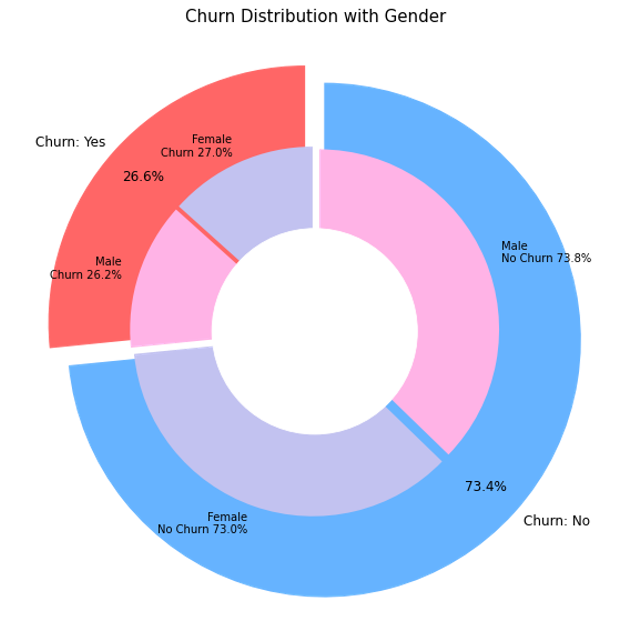
\includegraphics[width=0.78\columnwidth]{fig1-churn-by-gender.png}
\caption{Churn distribution by gender. The outer ring splits the 7,043 customers into churned and retained; the inner ring splits each group by gender, labeled with that gender's rate. The chart rounds the exact shares (26.54\% overall, 26.92\% of women, 26.16\% of men) to 26.6\%, 27.0\% and 26.2\%.}
\label{fig:gender}
\end{figure}

Two properties of the file shape every later modeling choice:
\begin{enumerate}
\item \textbf{The churn label has no date.} The dataset card describes churners as customers who left in the last month, but the file contradicts that reading. This study reads churn as leaving at some point during the recorded tenure, and states it as an assumption.
\item \textbf{No price ever changed.} Total charges divided by monthly charges times tenure has a median of 1.000, so every customer paid the same bill each month. Price sensitivity therefore cannot be estimated from these data, a point Section~\ref{sec:engine1} returns to.
\end{enumerate}

\subsection{Recovering the Price List}

Bills are not itemized, but the customers hold only 322 distinct combinations, or baskets, of ten services. Regressing each monthly bill on the customer's 0/1 service vector $\mathbf{a}_i$ recovers one price per service, $P^0$, with $R^2 = 0.9988$ and a residual standard deviation of \$1.02. The residuals are uncorrelated with tenure and with churn, so the fit does not hide a pricing history.
\begin{equation}
B_i(P) = \mathbf{a}_i^{\top} P, \qquad B_i^{0} = \mathbf{a}_i^{\top} P^{0}
\label{eq:bill}
\end{equation}

The recovered list prices a phone line at \$20.05, DSL at \$25.05 and fibre at \$50.01, with each smaller add-on near \$5 and each streaming service near \$10 (the Overview page in Section~\ref{sec:ui} lists all ten). Because bills are linear in prices, any candidate price list maps exactly to every customer's new bill. It also means a bill-shock limit needs one row per basket rather than one per customer, which cuts 7,043 two-sided limits to 322.

\subsection{Monthly Churn Hazard}
\label{sec:hazard}

Both engines need a monthly probability of leaving, not an ever-left flag. A piecewise-exponential survival model provides it~\cite{b9}. Each customer's history is split into months at risk within five tenure bands (1--6, 7--12, 13--24, 25--48 and 49--72 months), which yields 227,990 customer-months and 1,869 events.

A Poisson generalized linear model on these counts, with exposure as the weight, is equivalent to the piecewise-exponential likelihood~\cite{b10}. It is fit with scikit-learn's \texttt{PoissonRegressor} without a penalty, and it matches the textbook log-offset formulation to $2\times10^{-15}$. Customer $i$'s current hazard is
\begin{equation}
h_i = \exp\!\left(\beta_{b(i)} + \boldsymbol{\beta}^{\top}\mathbf{z}_i\right)
\label{eq:hazard}
\end{equation}
where $b(i)$ is the band of the customer's current tenure. The covariates $\mathbf{z}_i$ are contract type, payment method, the ten service indicators, paperless billing, senior-citizen status, partner and dependents.

The mean monthly hazard is 2.18\% and the median 0.89\%. The hazard ratios that Engine~2 later uses are 0.21 for a one-year contract, 0.055 for a two-year contract, 0.65 for tech support, 0.52 for online security and 0.52 for card autopay. These are associations in observational data: customers who chose long contracts may have been less likely to leave in any case, and no offer was ever made in this dataset.

The model has one known flaw. It misses the lock-in of two-year contracts, predicting 14.1 departures in their first 24 months where the data show none. Refitting with contract-by-band interactions repairs the fit, and it moves Engine~1's fibre cut only from 17.9\% to 18.4\%, so the main model is kept.

\subsection{Customer Lifetime Value}

Both objectives value a customer the same way. With monthly margin $\pi_i = m B_i$, a constant hazard $h_i$, a monthly discount rate $d$ and cash received at the end of each month, lifetime value is a geometric series:
\begin{equation}
\mathrm{CLV}_i = \sum_{t \ge 1} \frac{\pi_i (1-h_i)^{t-1}}{(1+d)^{t}} = \frac{\pi_i}{d + h_i}
\label{eq:clv}
\end{equation}

The defaults are $m = 70\%$ and $d = 1\%$ per month. At the average bill of \$64.86 and the mean hazard, a customer is worth about \$1,430. Because $h_i$ sits in the denominator next to a small $d$, halving a customer's hazard raises their value sharply, and both engines exploit that sensitivity.

\subsection{Engine 1: Price Optimization}
\label{sec:engine1}

Engine~1 chooses one monthly price per service, $P \in \mathbb{R}^{10}$, to maximize total lifetime profit over all 7,043 customers. A price rise earns more each month but shortens the expected stay, so each customer's hazard responds to the change in their bill:
\begin{equation}
h_i(P) = h_i \left( \frac{B_i(P)}{B_i^{0}} \right)^{\eta}, \qquad C_i = (1-m)\,B_i^{0}
\label{eq:response}
\end{equation}

Here $C_i$ is the monthly cost to serve, held at today's level, and $\eta$ is price sensitivity. No price changed in the data, and the fitted price coefficient flips sign across model specifications, so $\eta$ cannot be estimated. It is a scenario input, 0.8 by default and swept from 0.4 to 1.5. The engine solves
\begin{equation}
\begin{aligned}
\max_{P}\quad & Z(P) = \sum_{i=1}^{N} \frac{B_i(P) - C_i}{d + h_i(P)} \\
\text{s.t.}\quad & 0.75\,P_k^{0} \le P_k \le 1.25\,P_k^{0}, \quad k = 1,\dots,10 \\
& 0.85\,B_s^{0} \le \mathbf{u}_s^{\top} P \le 1.15\,B_s^{0}, \quad s = 1,\dots,322 \\
& P_{\mathrm{fibre}} - P_{\mathrm{DSL}} \ge 10 \\
& \tfrac{1}{N}\textstyle\sum_{i=1}^{N} h_i(P) \le \bar{H}
\end{aligned}
\label{eq:nlp}
\end{equation}
where $\mathbf{u}_s$ is the service vector of basket $s$ and $\bar{H} = 2.1774\%$ is today's mean monthly hazard. Each constraint has a stated purpose:
\begin{itemize}
\item \textbf{Price bounds ($\pm 25\%$)} keep the answer inside the range where a single $\eta$ is plausible. They are a modeling guard, not a market fact.
\item \textbf{Bill-shock limits ($\pm 15\%$ per basket)} stop any customer's bill from jumping, which in practice drives complaints. They form 644 linear inequalities.
\item \textbf{The tier gap} keeps fibre at least \$10 above DSL, so the faster product never becomes the cheaper one.
\item \textbf{The churn ceiling} is a management rule: repricing may not raise average churn. It is the only nonlinear constraint, and Section~\ref{sec:res-e1} shows that it decides the answer.
\end{itemize}

An earlier draft also carried a bundle-discount constraint. With additive bills it compared a sum to 90\% of itself and could never bind, so it was removed.

The objective is a sum of ratios, a fractional program that is not concave in general. The ceiling is convex in $P$ when $\eta \ge 1$ and concave when $\eta < 1$, so the engine treats (\ref{eq:nlp}) as a general smooth nonlinear program. It is solved with sequential least-squares quadratic programming (SLSQP)~\cite{b13} as implemented in SciPy~\cite{b15}.

Analytic gradients are supplied for the objective and every constraint, and the objective is divided by today's profit so its values stay near one. The solver runs from eight starting points, today's prices plus seven random lists within $\pm 10\%$, and a result is accepted only when all eight agree. The Lagrange multiplier on the ceiling, taken from the Karush--Kuhn--Tucker (KKT) conditions, gives the value of extra churn room.

\subsection{Engine 2: Retention Offer Assignment}
\label{sec:engine2}

Engine~2 decides which at-risk customers to call and with which of six offers (Table~\ref{tab:offers}). Candidates are the 740 current customers whose monthly hazard is at least 3\%.

Only current customers can be called, so the 911 customers at that risk who have already left are excluded, while the hazard model still learns from all 7,043 records. Engine~1 keeps pricing every customer, because a price list applies to the whole base.

\begin{table*}[!t]
\caption{Retention Offers}
\label{tab:offers}
\centering
\footnotesize
\setlength{\tabcolsep}{4pt}
\begin{tabular}{@{}L{2.7cm}L{3.0cm}L{2.9cm}L{1.4cm}L{1.6cm}L{1.2cm}L{3.4cm}@{}}
\toprule
\textbf{Offer} & \textbf{Customer receives} & \textbf{Hazard ratio during term} & \textbf{Term} & \textbf{Cost if accepted$^{a}$} & \textbf{Agent time} & \textbf{Eligible customers} \\
\midrule
One-year contract & 10\% off & 0.21 & 12 mo & \$77.83 & 0.5 h & Month-to-month \\
Two-year contract & 15\% off & 0.055 & 24 mo & \$233.49 & 0.75 h & Month-to-month or one-year \\
Free tech support & 6 months free & 0.65 & 6 mo & \$9.05 & 0.5 h & Internet, no tech support \\
Free online security & 6 months free & 0.52 & 6 mo & \$9.02 & 0.5 h & Internet, no security \\
Autopay switch & \$25 credit & 0.52 & Permanent & \$25.00 & 0.5 h & Pays by electronic or mailed check \\
Two-year + tech support & Both, plus a \$10 bundle cost & Both for 6 mo, then 0.055 & 24 mo & \$252.54 & 1.0 h & Meets both eligibilities \\
\bottomrule
\end{tabular}\\[3pt]
\parbox{\textwidth}{\scriptsize $^{a}$At the average bill of \$64.86 a month. Hazard ratios are relative to a customer without the attribute.}
\end{table*}

An offer replaces the customer's hazard $h_i$ with $h'_{ij}$, the hazard from (\ref{eq:hazard}) with the offered attribute switched on, for the offer's term $L_j$. The hazard then returns to $h_i$. With $q = (1 - h'_{ij})/(1 + d)$, the lifetime value along that path, the offer's expected value and its expected cost are
\begin{equation}
\mathrm{CLV}_{ij} = \frac{\pi_i}{1+d}\cdot\frac{1-q^{L_j}}{1-q} + q^{L_j}\,\frac{\pi_i}{d+h_i}
\label{eq:clvoffer}
\end{equation}
\begin{equation}
V_{ij} = \alpha\left(\mathrm{CLV}_{ij} - \frac{\pi_i}{d+h_i}\right), \qquad c_{ij} = \alpha\,\kappa_{ij}
\label{eq:value}
\end{equation}
where $\kappa_{ij}$ is the cost if accepted and $\alpha = 30\%$ is the acceptance rate. The acceptance prior follows the churn-profit literature, which models it as Beta(6,~14) with mean 0.3~\cite{b3}. A discount costs the revenue given up, while a free service costs its unit cost for six months. Money is spent only when a customer accepts, so it is weighted by $\alpha$, but agent hours $t_j$ are spent on every call.

The assignment problem is
\begin{equation}
\begin{aligned}
\max_{x}\quad & \textstyle\sum_{i}\sum_{j} V_{ij}\,x_{ij} \\
\text{s.t.}\quad & \textstyle\sum_{j} x_{ij} \le 1 \quad \forall i \\
& \textstyle\sum_{i}\sum_{j} c_{ij}\,x_{ij} \le 30{,}000 \\
& \textstyle\sum_{i}\sum_{j} t_{j}\,x_{ij} \le 500 \\
& \textstyle\sum_{i} x_{ij} \le 350 \quad \forall j \\
& x_{ij} \in \{0,1\}
\end{aligned}
\label{eq:bip}
\end{equation}

Only eligible pairs with positive value enter the model: 3,952 binary variables and 748 constraints (740 choice rows, the budget, the hours and six caps). The structure is a multiple-choice multidimensional knapsack problem, which is NP-hard in general~\cite{b16}. Here only eight rows link customers together, so the linear-programming (LP) relaxation is nearly integral.

The model is solved with HiGHS~\cite{b17} through SciPy's \texttt{milp} interface, which runs branch and bound with cutting planes. It stops at a 0.1\% optimality gap or a 30\,s time limit, raised to 180\,s on the hosted server. The LP relaxation supplies a certified upper bound, and three greedy rankings (value per dollar, value per resource and raw value) serve as baselines.

\subsection{Coupling the Engines}
\label{sec:coupling}

The engines meet at the churn ceiling. Engine~2 lowers the hazard of the customers it calls, which lowers the mean hazard and leaves room under Engine~1's ceiling. The coupling sweep measures that room for budgets $b$ of \$0, \$15,000, \$30,000, \$60,000 and \$90,000:
\begin{enumerate}
\item Solve Engine~2 at budget $b$ with $b/60$ agent hours and a cap of $b/85.7$ per offer, the same ratios as the \$30,000 campaign.
\item Convert each called customer's offer value into the constant hazard that yields the same lifetime value, using (\ref{eq:heq}).
\item Re-solve Engine~1 with these hazards while holding the ceiling at today's $\bar{H}$, and report the net gain (\ref{eq:gain}).
\end{enumerate}
\begin{equation}
h'_i = \frac{\pi_i}{\mathrm{CLV}_i + V_i} - d
\label{eq:heq}
\end{equation}
\begin{equation}
G(b) = Z\!\left(P^{*}, h'\right) - S(b) - Z\!\left(P^{0}, h\right)
\label{eq:gain}
\end{equation}
Here $S(b)$ is the expected retention spend and $Z(P^0, h) = \$17.01$M is today's lifetime profit. The procedure is a one-pass sequential decomposition rather than a joint optimum; Section~\ref{sec:res-coupling} discusses what that leaves out.

\subsection{Software Architecture}
\label{sec:arch}

The application has three tiers, each with one job (Fig.~\ref{fig:arch}). A React single-page interface displays results and never computes them. A Node.js server with no third-party packages validates requests, caches answers, runs background jobs and serves the built interface. Two long-lived Python processes hold the data and fitted models in memory and run the engines.

\begin{figure}[!t]
\centering
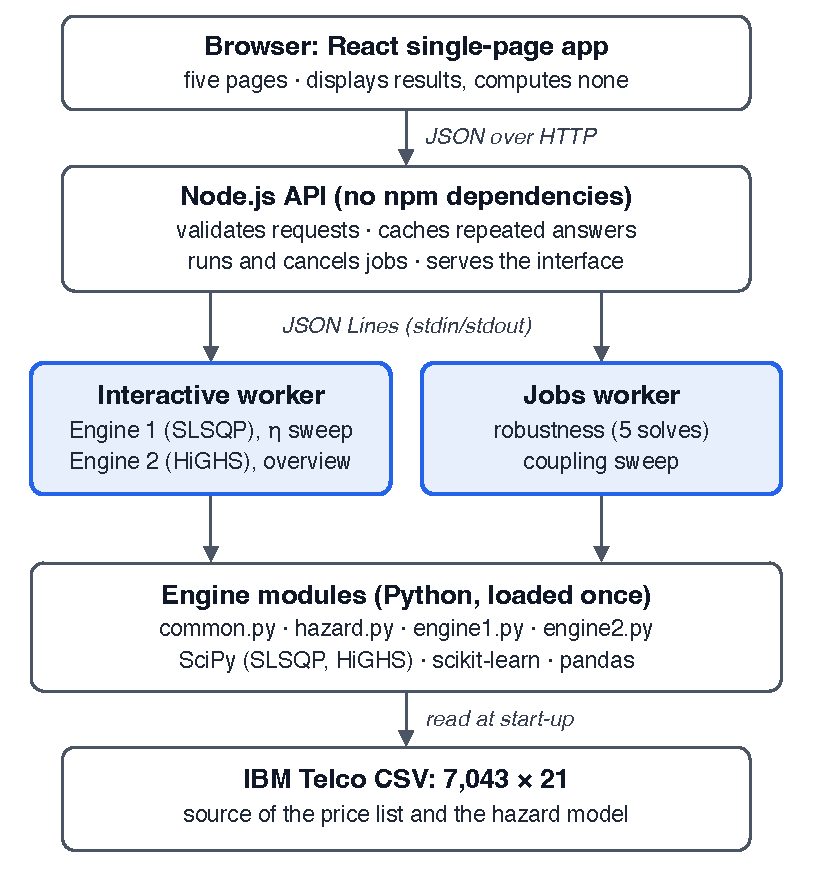
\includegraphics[width=\columnwidth]{fig2-architecture.pdf}
\caption{System architecture: React interface, dependency-free Node.js API, two persistent Python solver workers and the shared engine modules.}
\label{fig:arch}
\end{figure}

Keeping the models in memory means a solve starts within milliseconds instead of refitting the hazard model on every request. Multi-solve runs, the robustness check and the coupling sweep, go to the second worker as background jobs. Every integer solve also has a time limit, and a result cut short by it is flagged as the best found rather than proven optimal.

%======================================================================
\section{Implementation and Key Features}
\label{sec:impl}

The implementation keeps modeling, transport and presentation in separate code bases, bound by one rule: every number on screen arrives from the API. This section covers the technology stack (Table~\ref{tab:stack}), the interface and the model checks. The application is hosted publicly\footnotemark[1] and also runs on a laptop or in a Docker container.

\subsection{Technology Stack}

\begin{table}[!t]
\caption{Technology Stack}
\label{tab:stack}
\centering
\footnotesize
\setlength{\tabcolsep}{3pt}
\begin{tabular}{@{}L{1.15cm}L{2.25cm}L{1.45cm}L{3.3cm}@{}}
\toprule
\textbf{Layer} & \textbf{Technology} & \textbf{Version} & \textbf{Role} \\
\midrule
Interface & React & 19.2 & Components for the five pages \\
Interface & Vite & 8.3 & Development server and production build \\
Interface & Tailwind CSS & 4.3 & Styling, light and dark themes \\
API & Node.js & 20.19+ or 22.12+ & HTTP server, cache, job queue, static files \\
Engines & NumPy, pandas & 2.4.4, 3.0.2 & Data loading, price recovery, person-month expansion \\
Engines & SciPy & 1.17.1 & SLSQP for Engine~1; \texttt{milp} with HiGHS for Engine~2 \\
Engines & scikit-learn & 1.8.0 & Poisson model for the monthly hazard \\
Testing & Playwright & 1.63 & Browser tests in Chromium and WebKit \\
Delivery & Docker, Render, GitHub Actions & --- & Container image, hosting, continuous integration \\
\bottomrule
\end{tabular}
\end{table}

Python carries the modeling because SciPy offers both a sequential quadratic programming solver and the HiGHS mixed-integer solver behind one interface, and scikit-learn fits a Poisson model with exposure weights. The four numerical libraries are pinned, since the shadow price in Section~\ref{sec:results} relies on SLSQP's multipliers, which were confirmed on SciPy 1.17.1.

Node.js serves HTTP from its standard library alone, so the API needs nothing installed beyond Node. React with Vite gives fast rebuilds during development and a static bundle that the API serves in production.

\subsection{User Interface}
\label{sec:ui}

The interface has five pages behind a sidebar. Pricing, Retention and Coupling share one assumptions card holding $\eta$, the margin and the discount rate. A result computed under different settings is marked as stale rather than silently mixed with new inputs. All screenshots in this section come from the hosted application at its default settings.

\subsubsection{Overview} The Overview page summarizes the data before any optimization runs (Fig.~\ref{fig:overview}). It shows the customer count, the churn rate, the price-fit $R^2$, the 740 retention candidates, the recovered price list, churn by contract and the verification tally.

\begin{figure*}[!t]
\centering
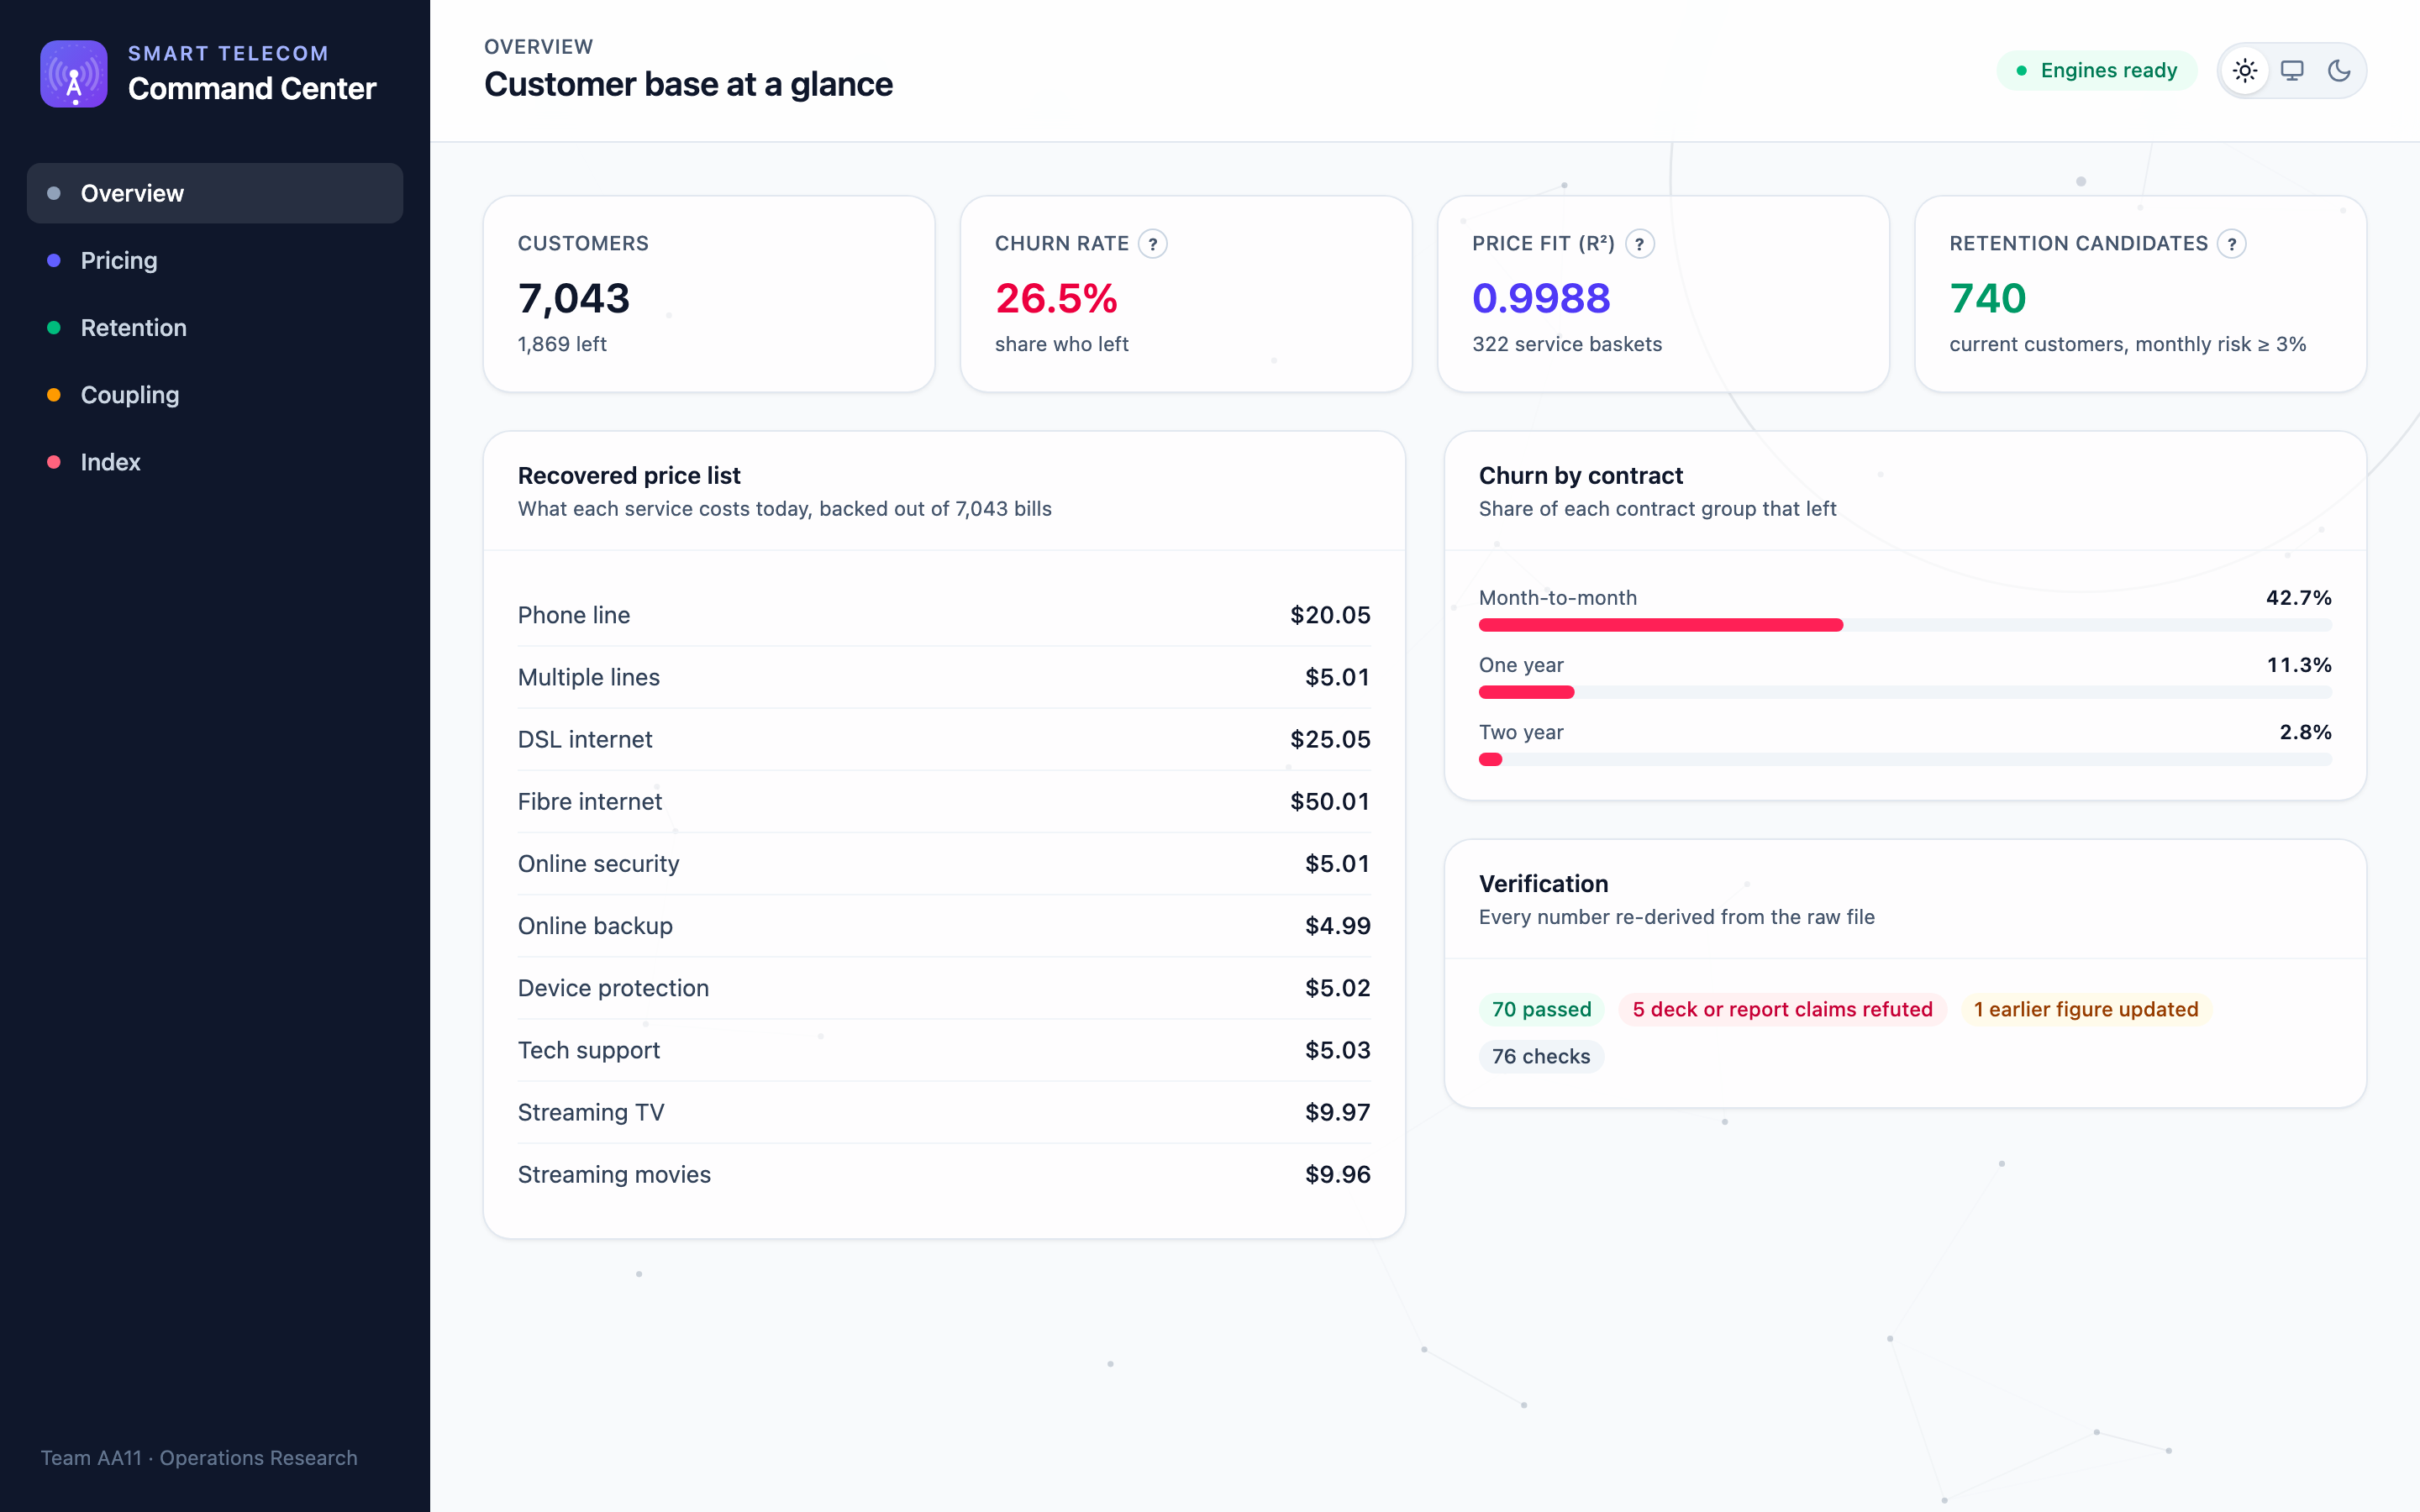
\includegraphics[width=0.9\textwidth]{fig3-overview.png}
\caption{Overview page of the hosted application: headline counts, the recovered price list, churn by contract and the verification tally (70 of 76 checks pass; the other six are refuted or updated earlier claims).}
\label{fig:overview}
\end{figure*}

\subsubsection{Pricing} The Pricing page runs Engine~1 and reports, for each service, the current and optimal price, the change, and the constraint that holds the price in place (Fig.~\ref{fig:pricing}). A sensitivity panel re-solves the model at four values of $\eta$ and compares the patterns of binding constraints.

\begin{figure}[!t]
\centering
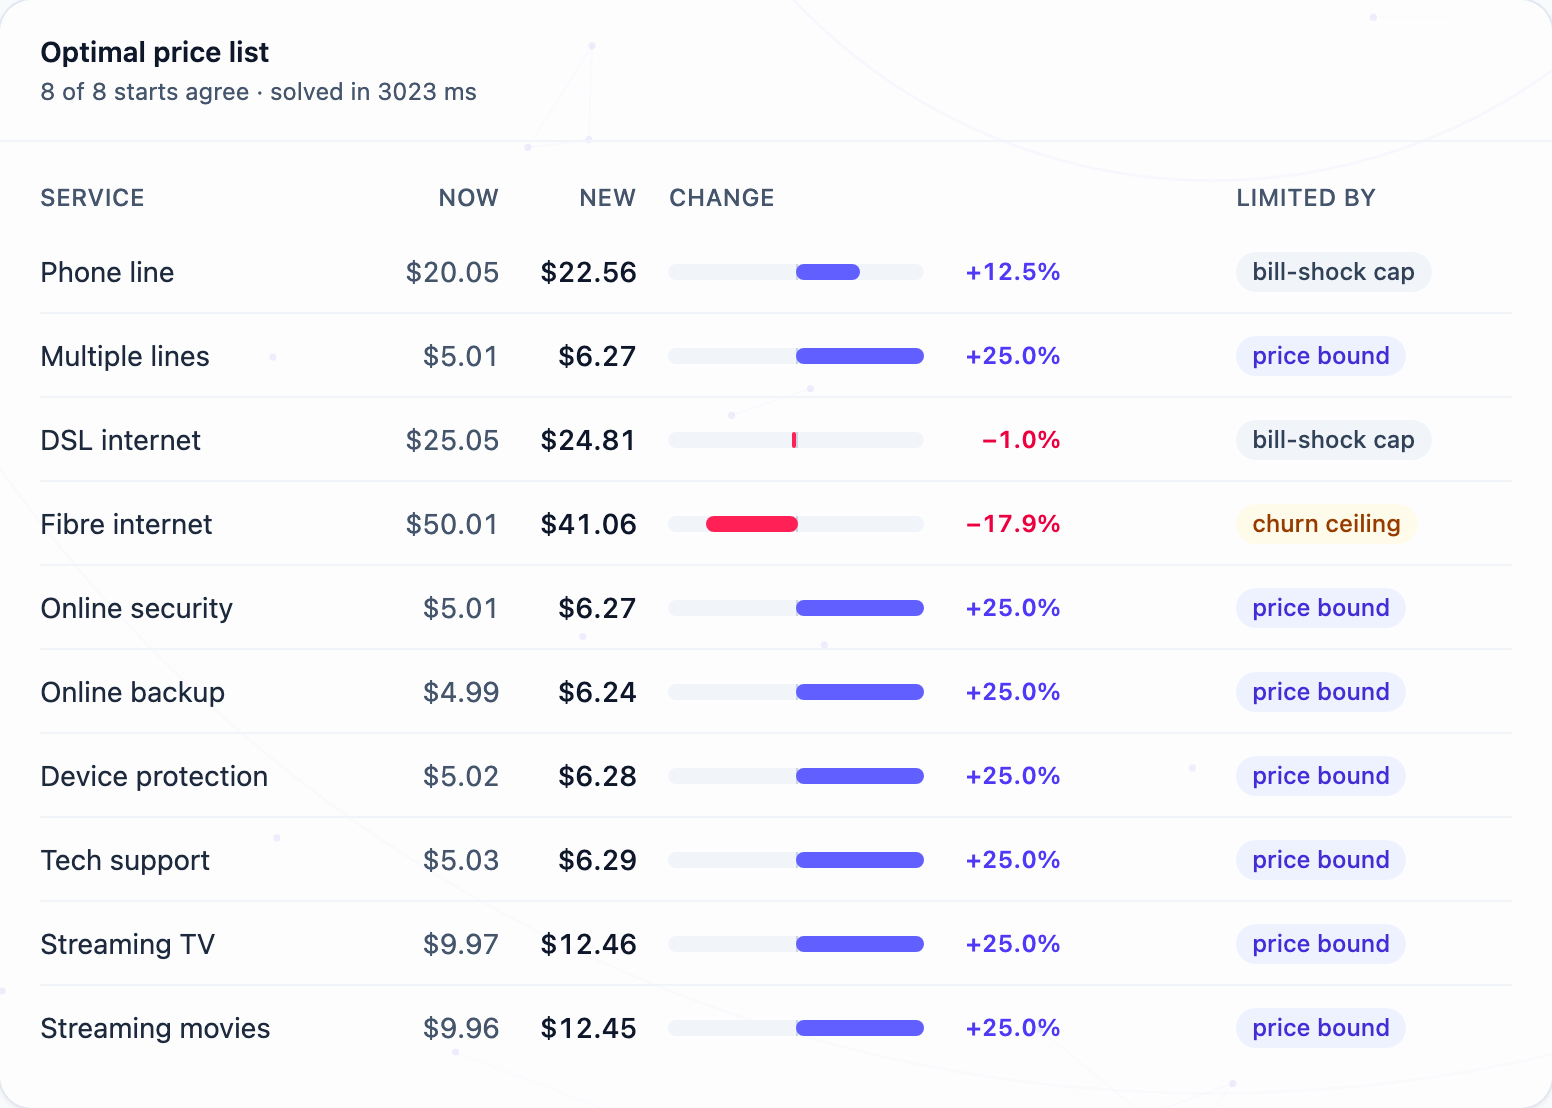
\includegraphics[width=\columnwidth]{fig4-pricing-table.png}
\caption{Optimal price list on the Pricing page. The Limited By column names each service's binding constraint; all eight starting points agree, and the solve took 3.0\,s on the hosted server.}
\label{fig:pricing}
\end{figure}

\subsubsection{Retention} The Retention page exposes the campaign settings: budget, agent hours, cap per offer, acceptance rate, risk threshold and a contract-effect strength. It reports the expected value with its LP bound, the offer mix, a robustness panel and the call list. The call list is sorted by expected value and exports to CSV for a call center (Fig.~\ref{fig:calllist}).

\begin{figure}[!t]
\centering
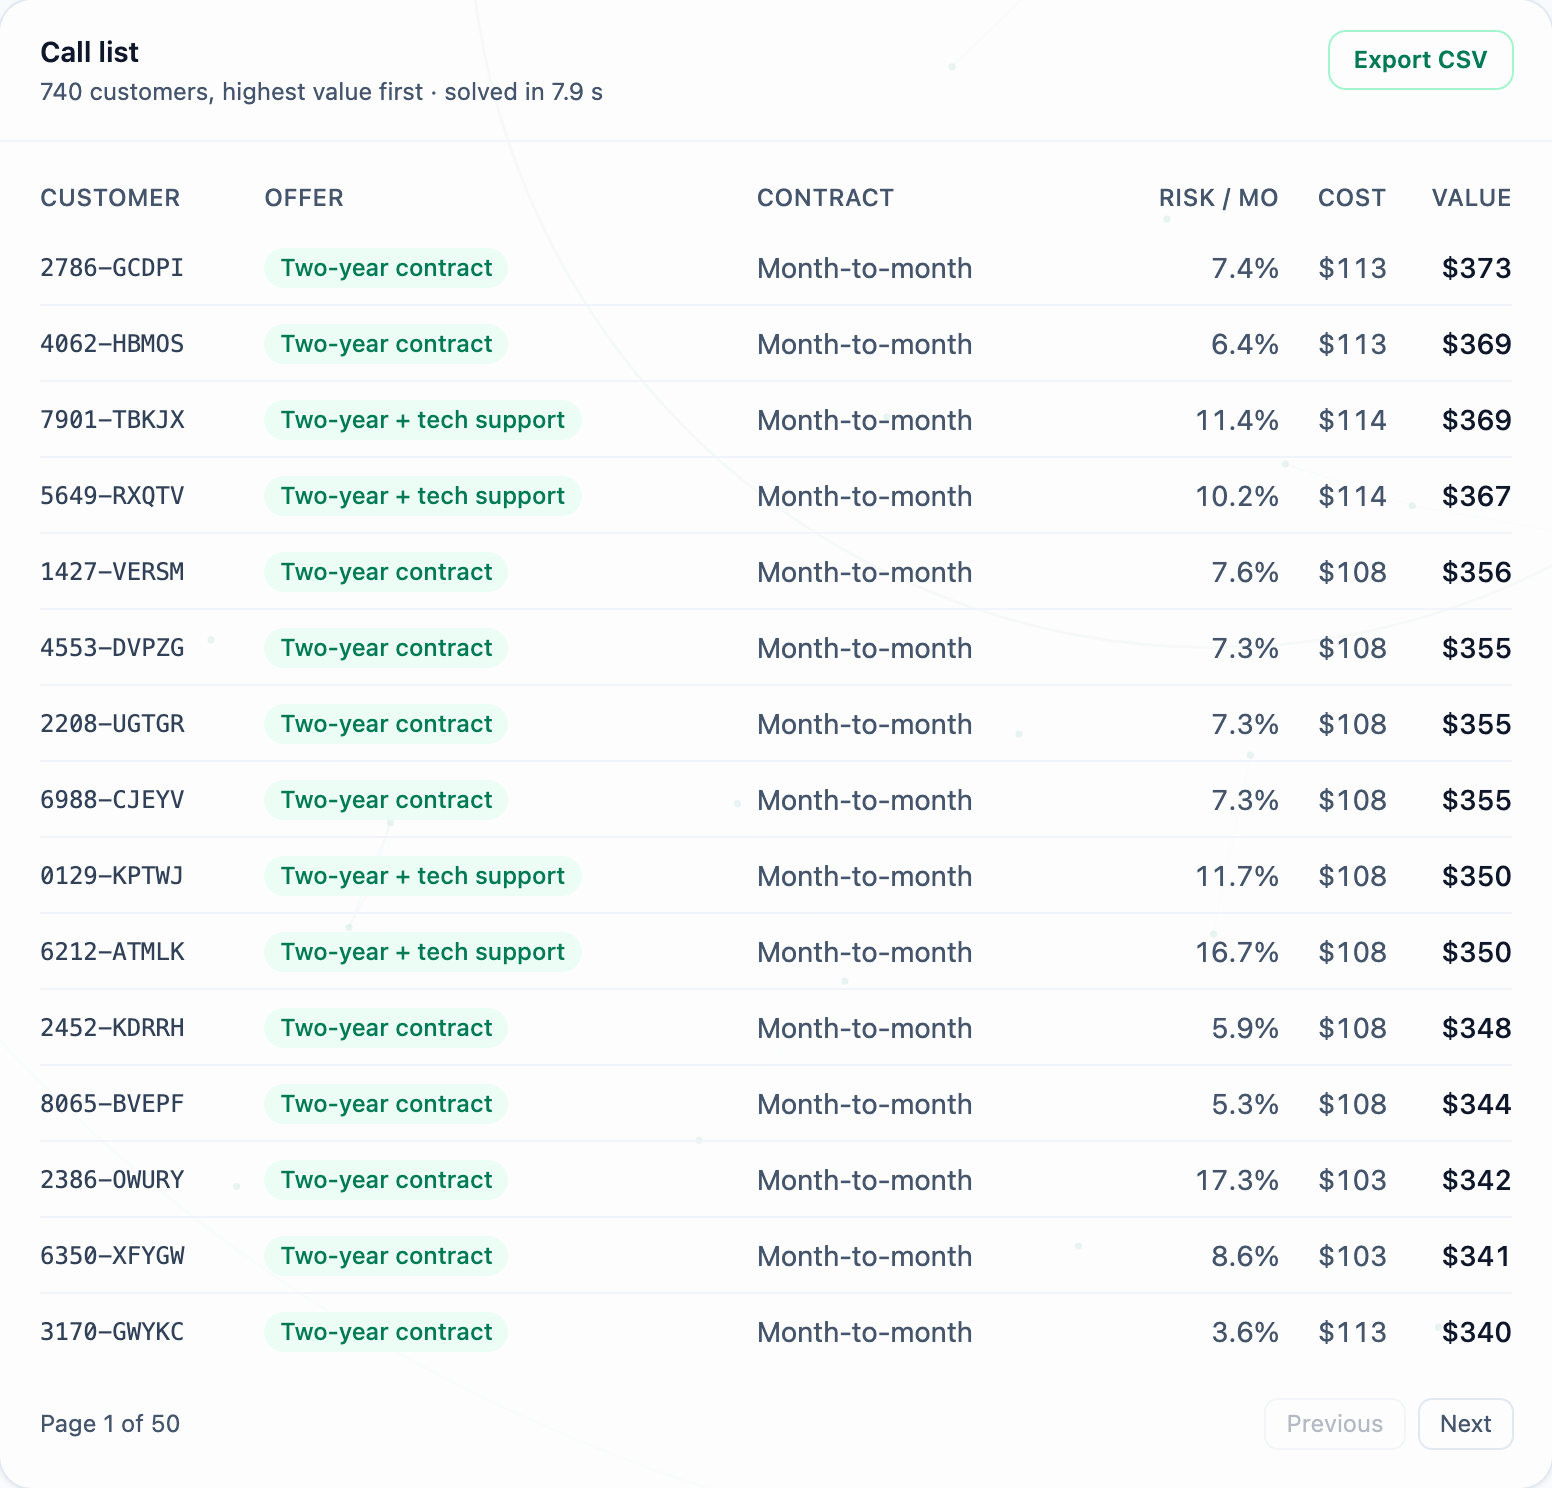
\includegraphics[width=\columnwidth]{fig5-call-list.png}
\caption{Call list on the Retention page: 740 customers sorted by expected value, with the assigned offer, contract, monthly risk, expected cost and value. Solved in 7.9\,s on the hosted server.}
\label{fig:calllist}
\end{figure}

\subsubsection{Coupling} The Coupling page accepts any comma-separated list of budgets and runs the sweep as a background job, with a progress bar and a Cancel button (Fig.~\ref{fig:coupling}). It plots the net gain against the budget and tabulates each run.

\begin{figure*}[!t]
\centering
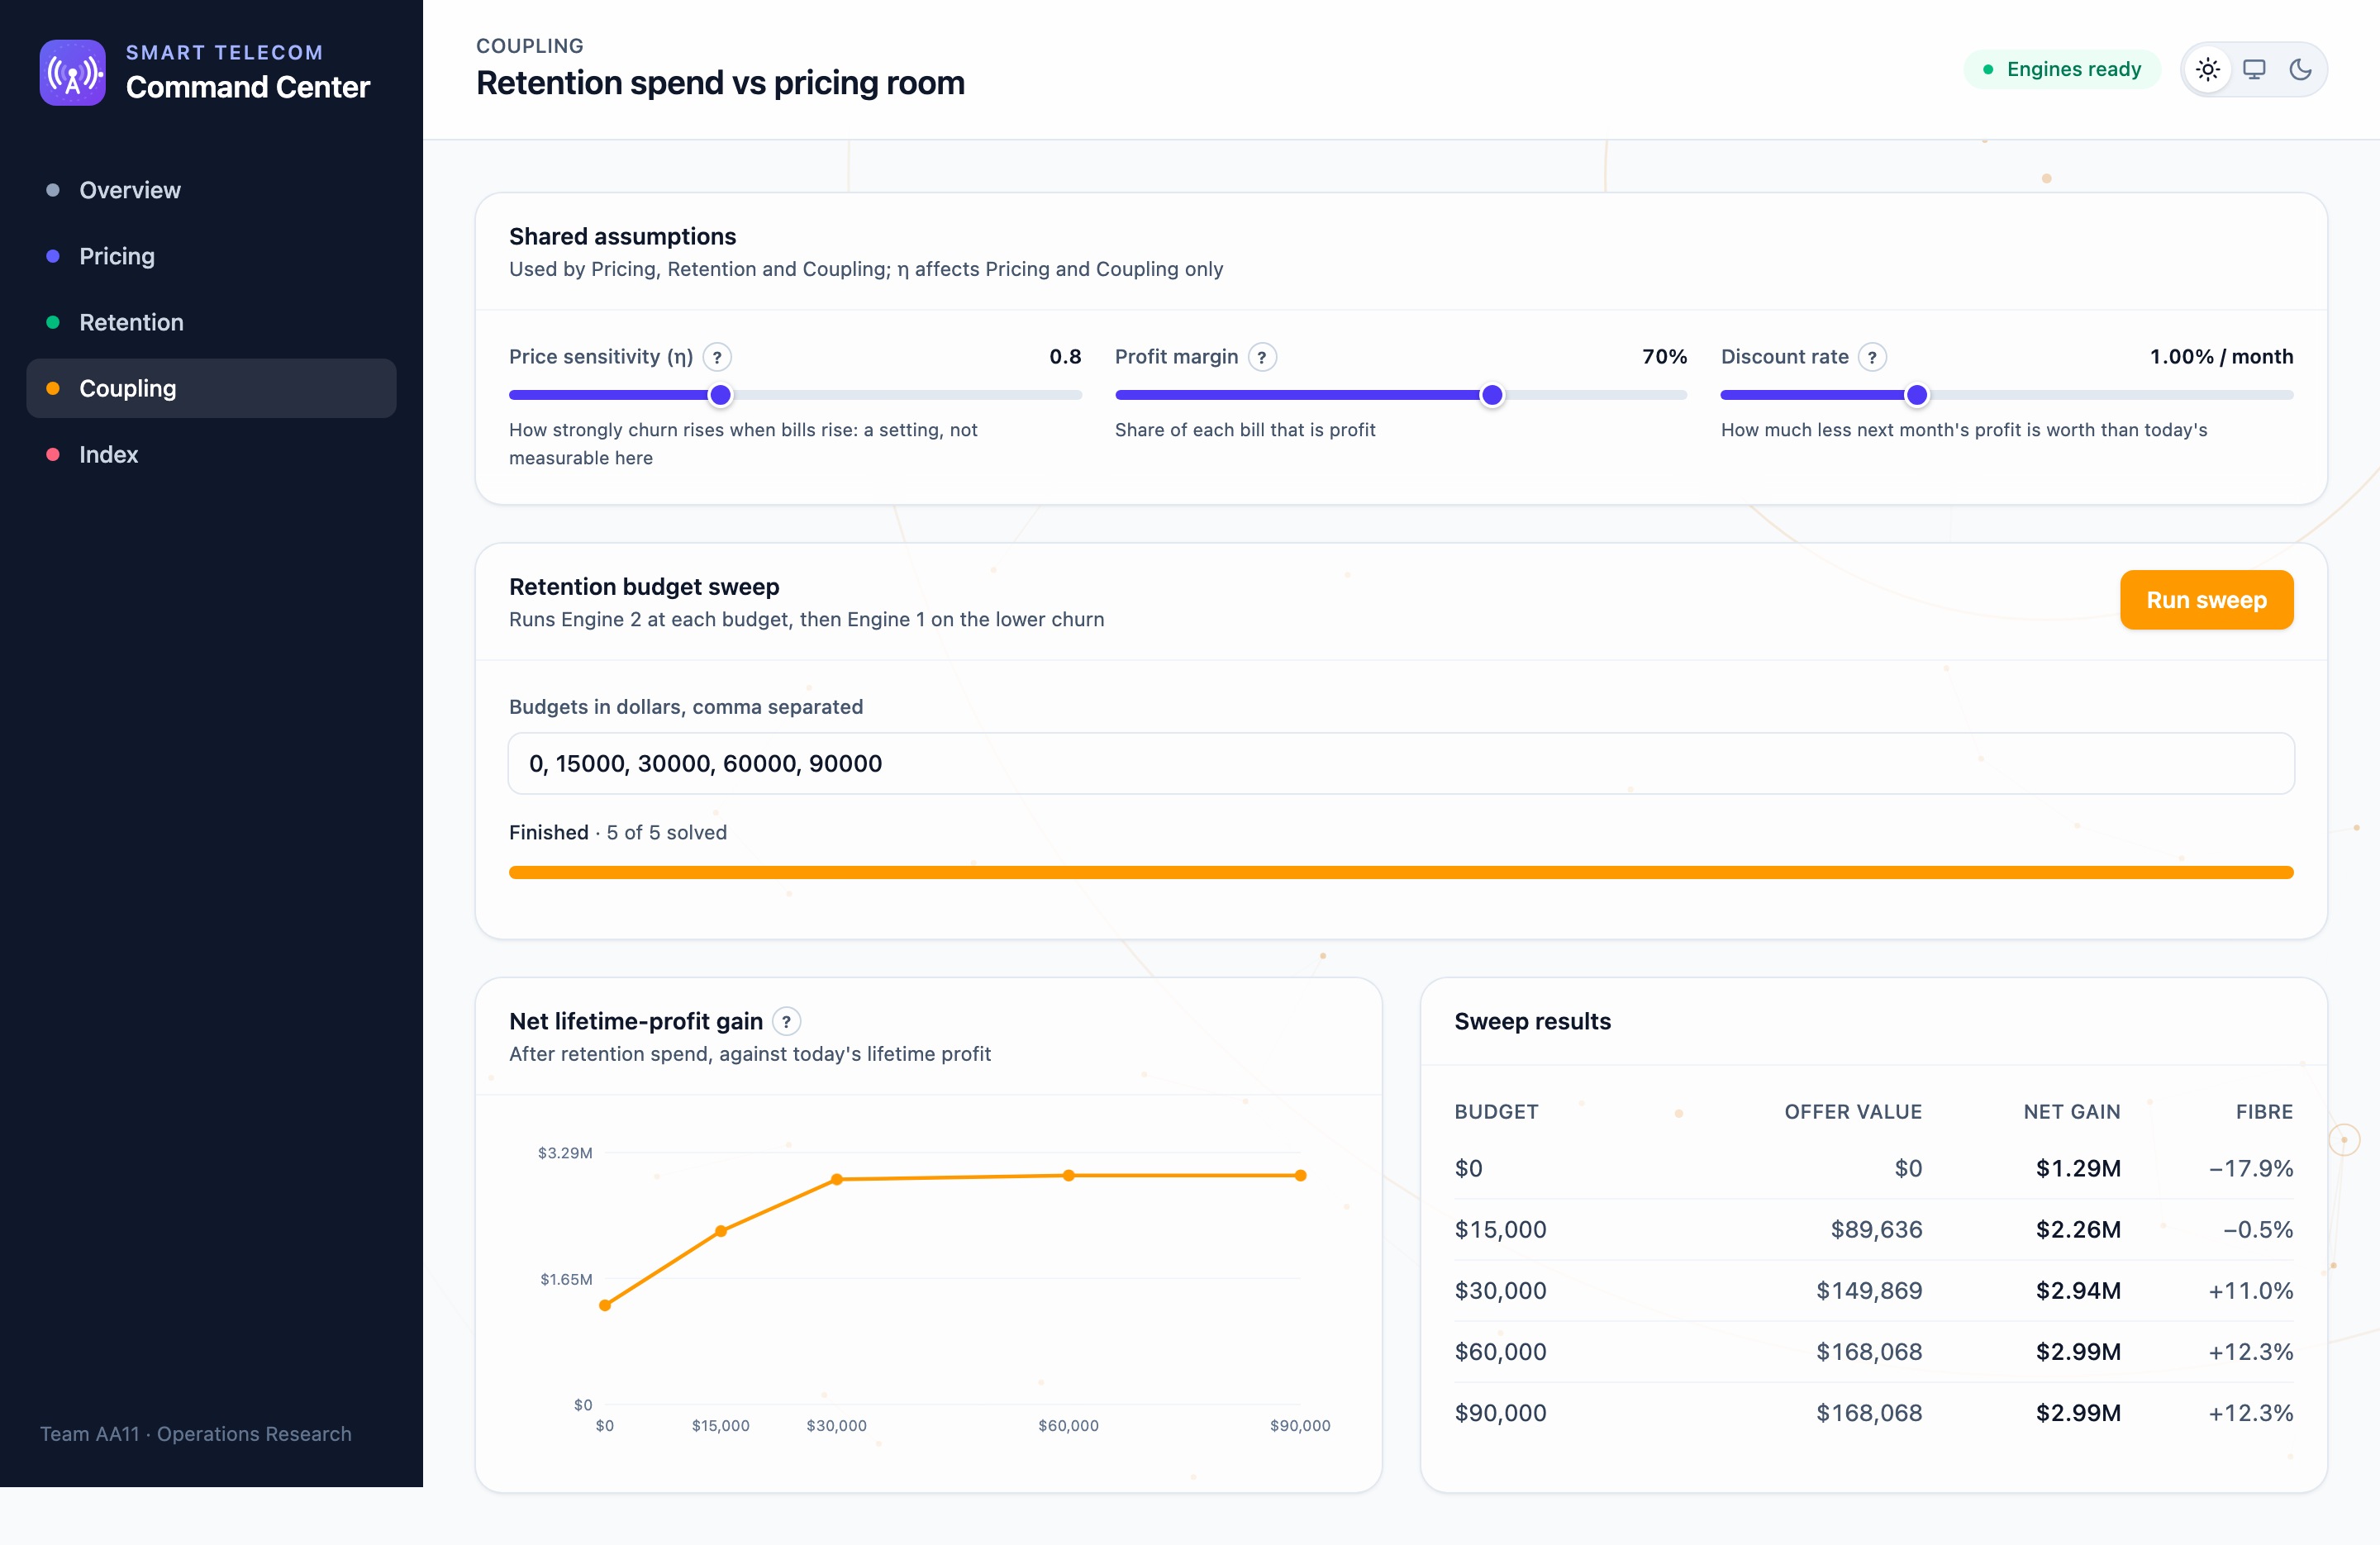
\includegraphics[width=0.86\textwidth]{fig6-coupling.png}
\caption{Coupling page of the hosted application after a five-budget sweep: shared assumptions, job progress, the net-gain curve and the sweep table at default settings.}
\label{fig:coupling}
\end{figure*}



\subsection{Model Verification}

\texttt{engine/verify.py} re-derives every reported figure, from the recovered price list to the coupling sweep, directly from the raw CSV in 76 checks across stages A--J. Section~\ref{sec:res-verify} reports the outcome.

%======================================================================
\section{Results and Discussion}
\label{sec:results}

All results come from the hosted application at its default settings: $\eta = 0.8$, a 70\% margin, a 1\% monthly discount rate and, for Engine~2, a \$30,000 budget, 500 agent hours, a cap of 350 per offer, 30\% acceptance and a 0.1\% optimality gap. Every monetary figure is an expected value under these settings, not a forecast.

\subsection{Engine 1: Repricing Under a Churn Ceiling}
\label{sec:res-e1}

Engine~1 raises revenue by 3.52\% and lifetime profit by 7.61\%, from \$17,013,333 to \$18,307,575, while the mean hazard stays exactly at today's level. All eight starting points reach the same prices, with a spread of $1.2\times10^{-12}$.

The price pattern in Fig.~\ref{fig:pricing} has a clear structure. Multiple lines and the six add-ons rise to their $+25\%$ bound. The phone line rises 12.5\% until the bill-shock limit on the phone-plus-multiple-lines basket binds, and DSL falls 1.0\% under the limit on the DSL-plus-all-add-ons basket. Fibre falls 17.9\%, from \$50.01 to \$41.06, and it is the one price held by the churn ceiling.

The ceiling, not the curvature of the objective, produces this answer. With the ceiling removed, every price climbs to the $+15\%$ bill-shock limit, profit reaches \$19.99M ($+17.5\%$) and mean churn rises to 1.118 times today's level. Every other increase raises some customers' hazard, and cutting fibre is the cheapest way the optimizer finds to buy that churn back.

The optimum also sits at a vertex. Eleven constraints are active for ten variables: seven upper price bounds, three bill-shock rows and the ceiling, with the third bill-shock row tight only because its basket is the sum of the other two. Margin and discount rate change the objective's scale but not the feasible region, so the optimal prices are identical for margins from 50\% to 90\% and discount rates from 0.5\% to 2\% a month.

\textit{Value of churn room:} The Lagrange multiplier on the ceiling values each extra 1\% of mean churn at \$164,816 of lifetime profit. Direct re-solves agree: loosening the ceiling by 1\% adds \$164,467, and tightening it by 1\% costs \$165,168. The figure prices the trade-off for management; it is not a recommendation to relax the rule.

\textit{Sensitivity to $\eta$:} Because $\eta$ cannot be measured, Engine~1 was re-solved at four values (Table~\ref{tab:eta}). The same constraints are active at every value, so the shape of the price list does not depend on $\eta$ within 0.4--1.5. At every value, multiple lines and the six add-ons sit at their $+25\%$ bound, the phone line and DSL are held by bill-shock limits, and fibre is held by the churn ceiling. Only the depth of the fibre cut and the size of the gain move. A higher $\eta$ makes each price rise cost more churn, so fibre must fall slightly further to keep the mean hazard at the ceiling.

\begin{table}[!t]
\caption{Engine 1 Sensitivity to Price Sensitivity $\eta$}
\label{tab:eta}
\centering
\footnotesize
\begin{tabular}{@{}lrrr@{}}
\toprule
$\boldsymbol{\eta}$ & \textbf{Revenue} & \textbf{Profit} & \textbf{Fibre} \\
\midrule
0.4 & $+3.61\%$ & $+8.08\%$ & $-17.65\%$ \\
0.8 (default) & $+3.52\%$ & $+7.61\%$ & $-17.89\%$ \\
1.2 & $+3.44\%$ & $+7.15\%$ & $-18.15\%$ \\
1.5 & $+3.37\%$ & $+6.81\%$ & $-18.34\%$ \\
\bottomrule
\end{tabular}
\end{table}

\subsection{Engine 2: Who to Call, With Which Offer}
\label{sec:res-e2}

Engine~2 calls all 740 candidates for an expected \$149,869 of preserved lifetime value (Fig.~\ref{fig:calllist}). The LP relaxation bounds any feasible list at \$149,872, so the solution is provably within 0.0021\% of optimal. The best of the three greedy rankings falls 8.25\% short.

The optimal mix uses three offers: the two-year contract for 350 customers (\$76,503), the autopay switch for 350 (\$61,726) and the two-year contract with tech support for 40 (\$11,640). The budget binds at \$29,998, and so do the caps on the two-year and autopay offers, while 477.5 of the 500 agent hours are used. Each call carries an expected cost of \$40.54 and about 39 minutes of agent time.

The LP relaxation is nearly integral: only four variables, spread over two customers, are fractional. Branch and bound needs to settle just those two, which is why the integer program solves in about half a second on a laptop. A greedy rule cannot weigh budget, hours and caps at once, and it cannot move a customer to a cheaper offer once a better offer's cap fills; the integer program does both.

The LP duals price the resources. An extra budget dollar is worth \$1.59 by the dual and \$1.42 by a direct re-solve at \$31,000; the gap arises because \$30,000 sits on a kink of a piecewise-linear value function. Agent hours have a zero dual, since 22.5 hours are spare.

\textit{Robustness:} The two softest inputs are the contract effects, which may partly reflect self-selection, and the acceptance rate. Engine~2 was re-solved with the log hazard ratio of each contract effect scaled by 0.5 and 0.25, and with acceptance at 15\% and 50\% (Table~\ref{tab:robust}).

\begin{table}[!t]
\caption{Robustness of the Call List}
\label{tab:robust}
\centering
\footnotesize
\setlength{\tabcolsep}{3.5pt}
\begin{tabular}{@{}lrrrrr@{}}
\toprule
\textbf{Case} & \textbf{Value} & \textbf{Change} & \textbf{Called} & \shortstack[r]{\textbf{Still}\\\textbf{called$^{a}$}} & \shortstack[r]{\textbf{Same}\\\textbf{offer$^{a}$}} \\
\midrule
Base (defaults) & \$149,869 & --- & 740 & --- & --- \\
Contract $\times 0.5$ & \$123,961 & $-17.3\%$ & 740 & 100.0\% & 85.1\% \\
Contract $\times 0.25$ & \$97,650 & $-34.8\%$ & 740 & 100.0\% & 75.4\% \\
Acceptance 15\% & \$78,597 & $-47.6\%$ & 699 & 94.5\% & 67.5\% \\
Acceptance 50\% & \$201,495 & $+34.4\%$ & 739 & 99.9\% & 55.2\% \\
\bottomrule
\end{tabular}\\[3pt]
\parbox{\columnwidth}{\scriptsize $^{a}$Still called: share of the base list called again. Same offer: share of those customers given the same offer. Contract $\times k$: log hazard ratio of each contract effect scaled by $k$.}
\end{table}

Who to call is robust: 94.5--100\% of the base list is called in every case. Which offer to make is less stable, since 55--85\% keep their offer as weaker contract effects shift customers between the two-year contract and the bundle. How much the campaign is worth is not robust at all, moving almost one for one with the assumptions. A campaign should therefore treat the call list as the firm output and the offer assignment as conditional on the contract-effect assumption.

\subsection{Coupling: Retention Spending Buys Pricing Room}
\label{sec:res-coupling}

The coupling sweep in Fig.~\ref{fig:coupling} shows that retention and pricing reinforce each other. With no campaign, repricing alone adds \$1.29M, which is Engine~1's answer from Section~\ref{sec:res-e1}. At \$15,000 the net gain rises to \$2.26M and the fibre cut almost disappears ($-0.5\%$), because the calls have lowered churn enough that the ceiling barely needs it.

At \$30,000 the campaign lowers the mean hazard by 9.1\%, fibre rises 11.0\% and the net gain reaches \$2.94M. Beyond about \$56,000 nothing more can be spent: every candidate already holds their best offer, so the \$60,000 and \$90,000 runs are identical, spending \$56,071 for a net gain of \$2.99M.

The returns fall quickly. Each budget dollar adds about \$65 of net gain over the first \$15,000, \$45 over the next \$15,000, \$1.75 from \$30,000 to \$60,000, and nothing after that. Past \$30,000 money stops being the scarce resource, and past \$56,000 the limit is the number of current at-risk customers.

Equations (\ref{eq:heq}) and (\ref{eq:gain}) also split the gain by source. The offers' own value net of their cost contributes $\$149{,}869 - \$29{,}998 \approx \$0.12$M at \$30,000; the remaining \$2.82M is repricing gain. Retention therefore earns most of its return indirectly: it buys \$1.52M of extra price room on top of the \$1.29M available with no campaign.

Two caveats bound this result. The sweep is a one-pass decomposition: Engine~2 chooses offers without knowing that prices will change, and Engine~1 treats the offers as fixed, so iterating the two engines or solving one mixed-integer nonlinear program could do better. The size of the gain also rests on the ceiling being a firm management rule; if it is not, the freed price room has no value.

\subsection{Performance}

Both engines solve in under a second on a laptop: Engine~1 takes about 0.3\,s for all eight starts, and Engine~2 about 0.5\,s, of which the LP bound takes 0.03\,s. On the hosted server, which has a tenth of a CPU, Engine~1 takes about 3\,s, Engine~2 about 8\,s and the five-budget coupling sweep about 28\,s.

\subsection{Verification Outcomes}
\label{sec:res-verify}

The solutions pass checks of feasibility, optimality and consistency. Engine~1's largest constraint violation is $1.4\times10^{-14}$, its eight starts agree, and its ceiling multiplier matches a $\pm 1\%$ re-solve within 0.3\%. Engine~2's chosen list satisfies every constraint when rechecked, and the LP bound proves it within 0.0021\% of optimal.

Multistart agreement is strong evidence that Engine~1 has found a global optimum, but not a proof, because the problem is not convex. For Engine~2 the bound is a proof: no feasible list can be worth more than \$149,872. Runs on macOS, Windows and Linux agree; the Windows runner finds \$149,866, within the 0.1\% gap.

Seventy of the 76 checks pass; the other six deliberately encode figures from an earlier draft that the data contradict, including the 26.6\% churn label in Fig.~\ref{fig:gender}.


\subsection{Limitations}
\label{sec:res-limits}

The results hold under assumptions that the data cannot test:
\begin{itemize}
\item \textbf{Price sensitivity is assumed.} No price changed in the data, so $\eta$ is a scenario input, and one value applies to every customer.
\item \textbf{Offer effects are associations.} The hazard ratios come from observational data and may partly reflect self-selection. Targeting by risk also ignores how differently customers respond to an offer~\cite{b5}; a randomized pilot would be needed to measure the effects.
\item \textbf{Expected values only.} Both engines optimize expectations, and uncertainty is handled by scenario re-solves rather than by stochastic or robust optimization.
\item \textbf{A single period.} Prices are set once and offers made once; nothing is re-optimized as customers respond.
\item \textbf{Fixed inputs.} Costs to serve are held at today's level, and offer terms, costs and agent hours are fixed in code rather than exposed as inputs.
\item \textbf{Near-optimal lists can differ.} At a 0.1\% gap, different machines may return different near-optimal call lists, and coupled net gains then differ by up to about 1\%. The hosted run's \$15,000 point (\$2.26M), for example, sits 0.15\% below a laptop run's (\$2.27M).
\end{itemize}

The system is therefore careful about what it claims. It never reports a measured price sensitivity, never states that an offer reduces churn by a fixed percentage, and presents \$149,869 as an expected value under stated settings rather than a promised saving.

%======================================================================
\section{Conclusion}
\label{sec:concl}

Pricing and retention act on the same quantity, the length of a customer's stay, and this work optimizes both on that common footing. On 7,043 IBM Telco customers, a nonlinear pricing model and a binary assignment model, joined through a ceiling on mean churn, turn a churn label and a set of stated assumptions into decisions a manager can inspect and challenge.

Three findings should carry beyond this dataset. First, the churn ceiling rather than the shape of the profit curve determines the optimal price list: seven prices rise to their bound and fibre falls 17.9\% to pay for them, for a \$1.29M gain in lifetime profit. Second, greedy targeting falls 8.25\% short of the integer program under the same budget, hours and caps, and the optimized call list survives weaker assumptions even when its offer assignments do not. Third, retention spending earns most of its return indirectly, by freeing pricing room: the first \$30,000 lifts the combined net gain from \$1.29M to \$2.94M.

The implementation shows one way to keep such models honest in software. Persistent solver workers sit behind a thin API, the interface displays only what the API returns, and 76 checks re-derive every figure while keeping refuted claims visible.

Future work follows from the limitations. A randomized pilot would replace the assumed offer effects and acceptance rate with measured ones, and a controlled price test would narrow the range of $\eta$. Iterating the two engines, or solving them as one mixed-integer nonlinear program, would show how much the sequential coupling leaves behind. A chance constraint on churn, a multi-period policy and support for an operator's own customer data would carry the system from demonstration toward deployment.

%======================================================================
\begin{thebibliography}{00}
\bibitem{b2} W. Verbeke, K. Dejaeger, D. Martens, J. Hur, and B. Baesens, ``New insights into churn prediction in the telecommunication sector: A profit driven data mining approach,'' \textit{Eur. J. Oper. Res.}, vol. 218, no. 1, pp. 211--229, Apr. 2012.
\bibitem{b3} T. Verbraken, W. Verbeke, and B. Baesens, ``A novel profit maximizing metric for measuring classification performance of customer churn prediction models,'' \textit{IEEE Trans. Knowl. Data Eng.}, vol. 25, no. 5, pp. 961--973, May 2013.
\bibitem{b4} S. A. Neslin, S. Gupta, W. Kamakura, J. Lu, and C. H. Mason, ``Defection detection: Measuring and understanding the predictive accuracy of customer churn models,'' \textit{J. Marketing Res.}, vol. 43, no. 2, pp. 204--211, May 2006.
\bibitem{b5} E. Ascarza, ``Retention futility: Targeting high-risk customers might be ineffective,'' \textit{J. Marketing Res.}, vol. 55, no. 1, pp. 80--98, Feb. 2018.
\bibitem{b9} M. Friedman, ``Piecewise exponential models for survival data with covariates,'' \textit{Ann. Statist.}, vol. 10, no. 1, pp. 101--113, Mar. 1982.
\bibitem{b10} T. R. Holford, ``The analysis of rates and of survivorship using log-linear models,'' \textit{Biometrics}, vol. 36, no. 2, pp. 299--305, Jun. 1980.
\bibitem{b13} D. Kraft, ``A software package for sequential quadratic programming,'' Inst. f\"{u}r Dynamik der Flugsysteme, DFVLR, Oberpfaffenhofen, Germany, Tech. Rep. DFVLR-FB 88-28, Jul. 1988.
\bibitem{b15} P. Virtanen \textit{et al.}, ``SciPy 1.0: Fundamental algorithms for scientific computing in Python,'' \textit{Nature Methods}, vol. 17, no. 3, pp. 261--272, Mar. 2020.
\bibitem{b16} H. Kellerer, U. Pferschy, and D. Pisinger, \textit{Knapsack Problems}. Berlin, Germany: Springer, 2004.
\bibitem{b17} Q. Huangfu and J. A. J. Hall, ``Parallelizing the dual revised simplex method,'' \textit{Math. Program. Comput.}, vol. 10, no. 1, pp. 119--142, Mar. 2018.
\end{thebibliography}

\end{document}
